\section{Silizium-PVD}
\label{siliconpvd}

Anhand von Silizium-PVD sollen einerseits amorphe Schichten abgeschieden, andererseits zur \ce{SiH4}-\ce{O2}-CVD hingeführt werden.
Nach Voruntersuchungen verschiedener ReaxFF-Para\-metrisierungen werden Abscheidungen auf kristallinen Silizium-Substraten unterschiedlicher Schnittebenen simuliert.
ASD

\subsection{Potentialdateien}

Für die folgenden Simulationen werden ReaxFF-Potentiale mit der Aussicht genutzt, auch Reaktionen zwischen Oberflächenatomen und Precursormolekülen simulieren zu können.
Da die ReaxFF-Formulierung erst innerhalb des letzten Jahrzehntes an Popularität gewonnen hat\todo{ref auf van Duin}, sind die verfügbaren Potentiale auf einzelne Probleme angepasst und oftmals noch nicht in den Potentialdatenbanken zu finden.
Tabelle~\ref{tab:siliconpotentials} listet die im Rahmen der Arbeit untersuchten ReaxFF-Parametrisierungen auf.

\begin{table}
  \caption[Silizium-Potentialdateien]{Potentialdateien für Silizium- und Siliziumoxidsysteme}
  \label{tab:siliconpotentials}
  \oddrowcolors
  \begin{tabularx}{1\textwidth}{|lXc|}
    \hline
    \textbf{Bezeichnung} & \textbf{Anwendung \& Kommentare} & \textbf{Ref.} \\
    \hline
    Al\_AlO\_AlN    & \ce{Al}, \ce{Al2O3}, \ce{AlN}. Basiert auf einer Si-Parametrisierung                                      & \cite{plimpton_lammps_2014} \\
    chenoweth       & Zersetzung von Polydimethylsiloxane bei hohen Drücken und Temperaturen. Ergänzung von \ce{C-Si}-Bindungen & \cite{chenoweth_simulations_2005} \\
    kulkarni        & Reaktion von Sauerstoff mit \ce{OH}-terminierten Siliziumoxid-Oberflächen                                 & \cite{kulkarni_oxygen_2013} \\
    lg              & ``low gradients''. Siehe liu\_nitramines. Fehlerhafte Version aus LAMMPS                                  & \cite{liu_reaxff-lg:_2011} \\
    liu\_ettringite & Verspannung von Ettringit (\ce{Ca6[Al(OH)6]2(SO4)3 26H2O}). Basiert auf Si-Parametrisierung               & \cite{liu_development_2012} \\
    liu\_nitramines & Dichtebestimmung von Nitramin-Molekülen bei hohen Drücken. Dichte erhöht durch Van-der-Waals-Korrekturen  & \cite{liu_reaxff-lg:_2011} \\
    narayanan       & Präparation mit \ce{Li-Al}-Silikaten. Für Phasenübergänge von Eukryptit-Kristallen (\ce{LiAl[SiO4]})      & \cite{narayanan_reactive_2012} \\
    newsome         & Oxidation von \ce{SiC}-Oberflächen mit \ce{O2} und \ce{H2O} bei \SIrange{500}{5000}{\kelvin}              & \cite{newsome_oxidation_2012} \\
    nielson         & Reaktionskinetik an Metallkatalysatoren bei hohen Temperaturen                                            & \cite{nielson_development_2005} \\
    zhang           & Zersetzung energetischer Moleküle (Nitramin-Explosionen)                                                  & \cite{zhang_carbon_2009} \\
    \hline
  \end{tabularx}
\end{table}

\subsection{Voruntersuchungen}

In Ergänzung zu den bisherigen Voruntersuchungen, die hauptsächlich aus Optimierungen und Relaxierungen von Kristallen bestanden, kommen hier auch Simulationen der Precursormoleküle für \ce{SiO2}-CVD, \ce{SiH4} und \ce{O2}, sowie der Oberfläche und amorpher Strukturen hinzu, wie sie bereits in Abschnitt~\ref{mdtests} vorgestellt wurden\todo{Hier beschreiben}.
Diese zusätzlichen Untersuchungen haben umfassendere Aussagen über die Anwendbarkeit der Parametrisierungen für vollständige Abscheidungssimulationen zum Ziel.
Lassen sich auch Reaktionen zwischen Precursormolekülen und der Oberfläche zuverlässig simulieren, könnte man die Precursormoleküle in Parsivald direkt auf der Oberfläche aufbringen, statt sie auf ihre Zentralatome zu reduzieren.
Die Ergebnisse dieser Betrachtungen wurden in Tabelle~\ref{tab:siliconpreresults} zusammen gefasst und im weiteren kurz diskutiert.

\begin{table}
  \begin{threeparttable}
    \caption[Ergebnisse der Silizium-Potential-Untersuchungen]{Zusammenfassung Ergebnisse der Untersuchung der Potentialuntersuchung für Silizium-Systeme.
      Detailliertere Ergebnisse finden sich in Anhang~\ref{appendix:silicon}
    }
    \label{tab:siliconpreresults}

    \oddrowcolors
    \begin{tabularx}{\textwidth}{|lCCCCCCC|}
      \hline
      \textbf{Bezeichnung}    & LMP    & c-\ce{Si} & c-\ce{SiO2} & a-\ce{Si} & \ce{SiH4} & \ce{+O2} & PVD\tnote{a} \\
      \hline                % & LAMMPS & c-Si      & c-SiO2      & a-Si      & Silane    & +O2      & PVD          \\
      Al\_AlO\_AlN            & \cmark & ~         & (\cmark)    &  \cmark   & \cmark    & ~        & \cmark       \\
      chenoweth               & ~      & ~         & ~           &  ~        & ~         & ~        & ~            \\
      kulkarni                & \cmark & \cmark    & \cmark      &  \cmark   & \cmark    & (\cmark) & \cmark       \\
      lg                      & ~      & ~         & ~           &  ~        & ~         & ~        & ~            \\
      liu\_ettringite         & \cmark & ~         & \cmark      &  \cmark   & ~         & ~        & \cmark       \\
      liu\_nitramines         & ~      & ~         & ~           &  ~        & ~         & ~        & ~            \\
      narayanan               & \cmark & ~         & \cmark      &  \cmark   & ~         & ~        & \cmark       \\
      newsome                 & \cmark & ~         & (\cmark)    &  ~        & ~         & (\cmark) & \cmark       \\
      nielson                 & \cmark & \cmark    & \cmark      &  \cmark   & \cmark    & ~        & \cmark       \\
      zhang                   & \cmark & ~         & ~           &  ~        & \cmark    & \cmark   & ~            \\
      \hline
    \end{tabularx}
    \todo[inline]{PVD Ergebnisse -> Anhang}

 %% & CVD\tnote{b}
 %% & CVD
 %% & \cmark?
 %% & ~
 %% & \cmark?
 %% & ~
 %% & \cmark?
 %% & ~
 %% & \cmark?
 %% & \cmark?
 %% & \cmark?
 %% & ~

    \begin{tablenotes}[para]
      \item[a] PVD: a-\ce{Si}-PVD mit Parsivald
      \item[b] CVD: a-\ce{SiO2}-CVD mit Parsivald
    \end{tablenotes}
  \end{threeparttable}
\end{table}

\subsubsection{Kompatibilität mit der Molekulardynamiksoftware (LMP)}

Einige Potentialdateien sind aus verschiedenen Gründen nicht mit der aktuellen Version der LAMMPS-Bibliothek kompatibel, was sich in harten Abbrüchen des Programmes äußert und sie von weiteren Untersuchungen ausschließt.
Andere Dateien lassen sich zwar laden und benutzen, äußern jedoch regelmäßige Warnungen über ihre van-der-Waals-Parameter, die aber nicht zu sonstigen Fehlern führen und meist nur Stickstoff- oder Platzhalteratome\footnote{Typischerweise beinhalten ReaxFF-Dateien wechselwirkungsfreie Platzhalterelemente unter dem Platzhalter-Element \ce{X} zum Zweck des Ausschlusses einzelner Partikel aus der Simulation} betrifft.

\subsubsection{Kristalleigenschaften (c-\ce{Si}, c-\ce{SiO2})}

Diese Untersuchungen decken sich mit dem bisherigen Vorgehen:
Eine Kristallstruktur wird unterhalb des Schmelzpunktes relaxiert, minimiert und anschließend hinsichtlich Koordination, Dichte und Bindungslänge analysiert.
Alle untersuchten Parametersätze erzeugen die korrekte Koordinationszahl von 4.0, mit klaren Spitzen in den radialen Verteilungsfunktionen und nahezu passenden Bindungslängen (Abbildung~\ref{fig:sisibondlengths}).
Der Newsome-Parametersatz generiert einen RDF-Peak vor der eigentlichen Bindungslänge, welcher der Vollständigkeit halber erwähnt sein soll, bei Bestimmung der Bindungslänge aus der RDF aber nicht über die Hauptbindungslänge dominiert.
Er führt bei amorphen Systemen jedoch zu einer Unterschätzung der Bindungslänge und Koordinationszahl (Tabelle~\ref{tab:amorphoussilicon}).
Im Allgemeinen stimmen die Kristalleigenschaften gut mit den erwarteten Werten aus der Standardliteratur überein.
Anhang~\ref{appendix:silicon} beinhaltet Abbildungen eines Vergleiches der Bindungslängen sowie eine exemplarische radiale Verteilungsfunktion des Kulkarni-Potentiales im kanonischen und im großkanonischen Ensemble.

\subsubsection{Amorphes Silizium (a-\ce{Si})}

Durch langsame Relaxation zufällig positionierter Siliziumatome wurde amorphes Silizium simuliert, das wie die Kristalle zuvor auf Dichte und Bindungslängen untersucht wurde.
Deren Werte variieren für amorphes Silizium stärker als für kristallines, liegen jedoch nah am experimentell bestimmten Wert von \SI{2.3}{\gpcc}\cite{remes_optical_1998}, anstatt Cluster und Hohlräume zu bilden.

\subsubsection{Stabilität der Precursormoleküle (\ce{SiH4}, \ce{O2})}

\todo[inline]{NVT? Bitte sag, dass kein kanonisches Ensemble benutzt wurde!}
ReaxFF-Potentiale versprechen die Simulation von Molekülen und deren Reaktion miteinander, die mit den folgenden Tests für Silan und molekularen Sauerstoff überprüft werden sollen.
Dazu wurden Simulationen einzelner und mehrerer Precursormoleküle (\ce{SiH4} und \ce{O2}) im kanonischen Ensemble bei verschiedenen Temperaturen simuliert und hinsichtlich ihrer Stabilität begutachtet.
Abbildung~\ref{fig:silanestability} zeigt eine Auswahl der Ergebnisse der Silan-Simulationen, an denen sich erkennen lässt, wie instabile Simulationen zur Ablösung der Wasserstoffatome vom Silanmolekül führen.

\subsubsection{Reaktion der Precursormoleküle (\ce{SiH4 + O2})}

\todo[inline]{NVT? Bitte sag, dass kein kanonisches Ensemble benutzt wurde!}
Reaktionen von einzelnen Precursormolekülen wurden stichprobenartig in verschiedenen Orientierungen, Energien und Temperaturen vorgenommen, um einen Überblick über die Verlässlichkeit zu bekommen.
Zusätzlich wurden durchmischte Precursorgase mit dem Ziel eventueller Reaktionen simuliert, was jedoch mit keiner der Parametrisierungen zum gewünschten Erfolg bei hoher Zuverlässigkeit führte.
Einige Parametrisierungen zeigen jedoch vielversprechende Teilreaktionen, die korrekte Doppelbindungen und Bildung von Wasserstoffmolekülen beinhalten (Abbildung~\ref{fig:precursorreactions}).
Vor allem bei größeren Reaktionsräumen bilden sich Cluster aus Precursormolekülen, die von attraktiven Termen in den Kraftfeldern dominiert werden, aber nicht durch chemische Wechselwirkungen zu erklären sind (Abbildung~\ref{fig:precursorclusters}).

\subsubsection{Abscheidungssimulationen (PVD, CVD)}

Die Abscheidungssimulationen selbst verlaufen wie in Kapitel~\ref{parsivald} vorgestellt und unterscheiden sich kaum von den Parsivald-Simulationen der vorherigen Abschnitte.
Als Ausgang werden amorphe und deshalb rauhere Schichten erwartet, die sowohl für \ce{Si}-PVD als auch \ce{SiO2}-CVD kontinuierlich wachsen, aber unterschiedlichen Bedingungen unterliegen.
Während die Silizium-Atome des PVD-Prozesses wie für Sputter-Prozesse üblich zufällig auf der Oberfläche auftreffen, finden die Reaktionen des CVD-Prozesses nur in der Nähe von auf der Oberfläche befindlichen Liganden statt.
Sauerstoff-Reaktionen werden also nur in der Nähe von Silan-Gruppen und Silan-Reaktionen nur in der Nähe von Hydroxyl-Gruppen oder Sauerstoffatomen generiert.

\subsection{Silizium-PVD}

Silizium-PVD dient in der Produktion elektronischer Artikel der Erzeugung einer dünnen, amorphen Siliziumschicht für unterschiedliche Anwendungsszenarien, für die konforme Schichten gleichbleibender Qualität gewünscht sind.
Durch den amorphen Charakter des Materials sind nanoskopische Leerstellen und höhere Rauheiten als bei monokristallinen Schichten zu erwarten, die im folgenden kurz untersucht werden sollen.
Rechenaufwendigere Rechenvorschriften des ReaxFF-Potentiales legen eine längere Simulationsdauer als bei EAM-Potentialen nahe, weshalb nur eine kleine Menge an Simulationen durchgeführt wurde.
Typische Laufzeiten von mehreren Wochen wurden für vollständige ReaxFF-Abscheidungssimulationen untersucht, jedoch sind im Gegensatz zu rein molekulardynamischen Untersuchungen größere Simulationsräume mit isolierten Ereignissen möglich, die eine Reduktion der Finite Size-Effekte zur Folge hat.

Als Substrat für die Parsivald-Simulationen wurden unrelaxierte Silizium-Monokristalle mit Oberflächen entlang der drei Kristallebenen (001), (011) und (111) präpariert und durch periodische Erweiterung auf \SI{106.416x103.68}{\angstrom} vergrößert.
Sonstige Parameter umfassen eine Temperatur von \SI{1300}{\kelvin} (der Schmelzpunkt liegt bei \SI{1687}{\kelvin}), Relaxationszeiten von \SI{350}{\femto\second} und MD-Box-Größen von \SI{37x37}{\angstrom}.
Die Auftreffenergie der Silizium-Atome liegt mit \SI{11.2}{\electronvolt} erneut vergleichsweise hoch, wird aber auch hier durch das Thermostat verringert\todo{wie weit?}.
Damit werden im Schnitt \num{1.68} parallele Ereignisse mit durchschnittlich \num{1510.65} Atomen und einer mittleren Laufzeit von \SI{60.71}{\second} berechnet.
Die Laufzeit lässt sich beispielsweise über die Zeitschrittweite noch minimieren, zeigt allerdings den Unterschied in der Laufzeit bei der Nutzung von EAM- und ReaxFF-Potentialen, der einem Faktor von etwa \num{12} für vergleichbare Operationen entspricht.
Die hohe Temperatur wurden gewählt, um Relaxationen zu beschleunigen, und übersteigen Temperaturen realer Abscheidungen.
Durch Justierung der Relaxationszeit, Zeitschrittweite, Thermostatdämpfung und Teilchenenergie lässt sich die Temperatur auf einen realistischeren Wert bei gleicher Verlässlichkeit der Simulation senken.

Das Ergebnis der Abscheidungssimulation ist eine vergleichsweise glatte, amorphe Siliziumschicht, die mit konstanter Rate wächst, jedoch eine Zunahme der Rauheit aufgrund von sich langsam verstärkenden Oberflächenunebenheiten aufweist.
Diese Unebenheiten wachsen im Gegensatz zu den Kupfer-Kratern aus Abschnitt~\ref{copperpvd} mit der Oberfläche entlang der Wachstumsrichtung, schließen sich aber ebenfalls selbsttätig, wenngleich über einen größeren Zeitraum.
Abbildung~\ref{fig:siliconresults-a} stellt dazu über der Simulationszeit neben der Schichtdicke die Rauheit dar, welche im Verlauf der Simulation stetig zunimmt und zuletzt einen RMS-Wert von \SI{1.15}{\nano\meter} annimmt, der experimentellen Erwartungen entspricht\todo{ref}.
Leider ermöglicht die begrenzte Laufzeit der Simulation ermöglicht keine Aussage über den weiteren Verlauf der Rauheit, von der sublinearer Verlauf durch Schließung der Unebenheiten erwartet wird, wie er sich bei den meisten Abscheidungsprozesse zeigt.\todo{ref?}

\begin{figure}
  \captionsetup[subfigure]{singlelinecheck=false}
  \def\subfigwidth{0.48\textwidth}
  \begin{subfigure}[t]{\subfigwidth}
    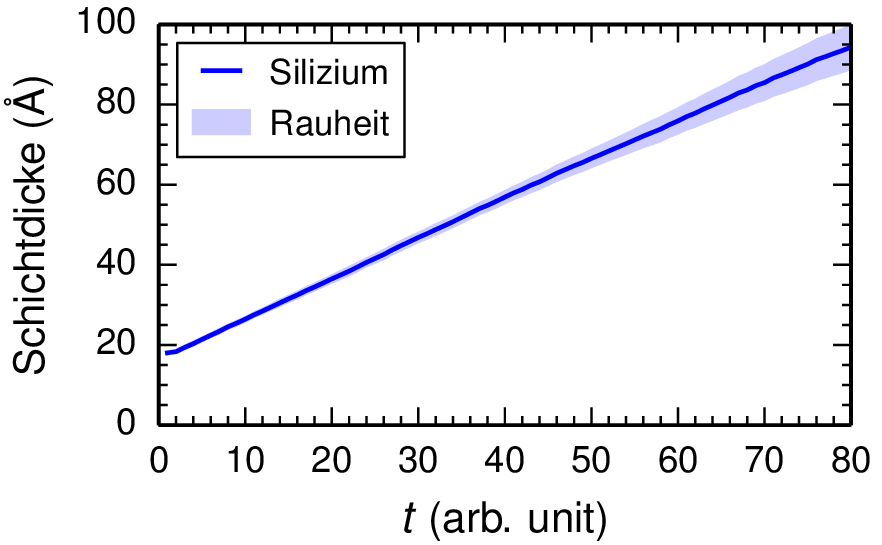
\includegraphics[width=\textwidth]{Si111_combined}
    \subcaption{Schichtdicke und Rauheit der aufgewachsenen Schicht}
    \label{fig:siliconresults-a}
  \end{subfigure}
  \begin{subfigure}[t]{\subfigwidth}
    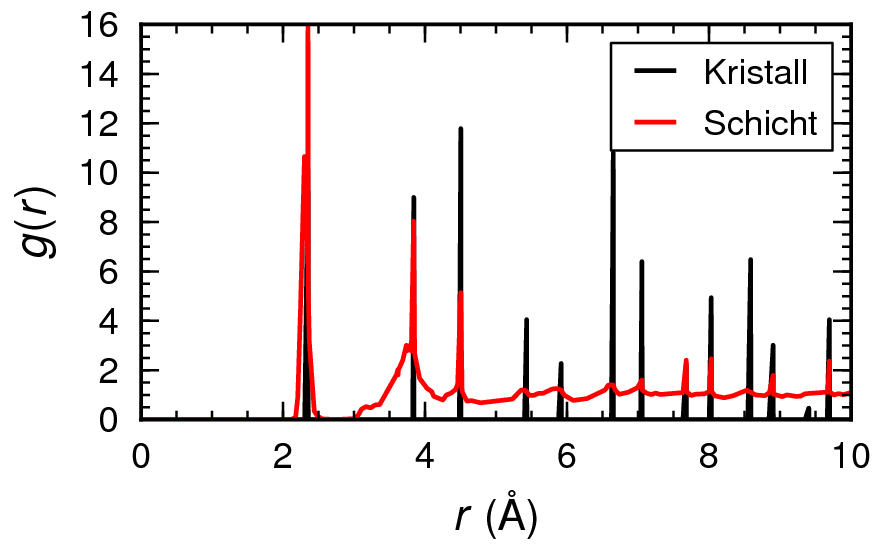
\includegraphics[width=\textwidth]{si111_rdf}
    \subcaption{Radiale Verteilungsfunktion der aufgewachsenen Schicht}
    \label{fig:siliconresults-b}
  \end{subfigure}
  \hfill
  \caption[Ergebnisse der Simulation einer Silizium-PVD]{Ergebnis der Simulation einer Silizium-PVD (\SI{10x10}{\nano\meter})}
  \label{fig:siliconresults}
\end{figure}

Abbildung~\ref{fig:siliconprofile} stellt die räumliche Verteilung der Unebenheiten dar, die sich lokal in Kratern und Poren von bis zu \SI{32}{\angstrom} Tiefe konzentrieren, aufgrund ihrer geringen Breite aber nur zu einer RMS-Rauheit von \SI{11.5}{\angstrom} führen.
Breitere Krater haben sich durch die geringe Größe des Simulationsraumes nicht entwickelt, jedoch wäre eine Untersuchung einer ca. \SI{500x500}{\angstrom} breiten Struktur auf deren Bildung interessant\todo{in den Ausblick packen?}.
Anhand des Profiles lässt sich auch erkennen, dass mitunter längere Relaxationszeiten oder höhere Teilchenenergien notwendig wären, um Porenbildung weiter zu verringern und langreichweitigere Unebenheiten zu befördern, wie sie etwa bei der Bildung nanoskopischer Silizium-Partikel gebildet würden.

Zum Vergleich beinhaltet Abbildung~\ref{fig:siliconunderrelaxedprofile} das Oberflächenprofil einer unterrelaxierten Oberfläche, wie sie während der Anpassung der Parsivald-Parameter entstanden sind.
Es zeigen sich stärkere Unterschiede und steilere Hänge, die sich aus der hohen Porösität des Materiales ergeben.
Somit ist zu erwarten, dass die Rauheit der Schicht mit stärkerer Relaxierung erwartungsgemäß weiter abnimmt.

\todo{Abschnitt viel weiter nach oben schieben}
Zur Charakterisierung der Kristalleigenschaften der abgeschiedenen Schicht wurden ihre RDF-Funktionen berechnet, aus denen ersichtlich ist, dass bereits nach \SI{4}{\angstrom}, also kurz vor der zweiten Korrelationslänge bei \SI{4.4}{\angstrom}, keine langreichweitige Ordnung mehr vorhanden ist.
Damit ist die Schicht amorph mit einer durchschnittlichen Koordinationszahl von \num{4}, woraus sich entnehmen lässt, \todo{wirklich?}dass die chemischen Bindungen
Die engen Spitzen an den charakteristischen Abständen des reinen Silizium-Kristalles werden durch das Substrat erzeugt, dass bei \SI{100}{\angstrom} Schichtdicke immerhin noch \SI{20}{\percent} der Struktur ausmacht, jedoch durch anfängliche Relaxierungen zum Teil seine Kristalleigenschaften verloren hat.

Anders als bei Gold oder Kupfer, bei denen metallische Bindungen dominieren, überwiegen in reinem Silizium \todo{wirklich?}kovalente Bindungen, so dass die mittleren Koordinationszahl von \num{3.99} anzeigt, dass alle 4 möglichen Bindungen der Siliziumatome tatsächlich ausgeprägt sind.
Somit zeigt sich die ReaxFF-Formulierung erfolgreich in der Darstellung der chemischen Eigenschaften von Silizium.

\begin{figure}[H]
  \centering
  \captionsetup[subfigure]{singlelinecheck=false}
  \begin{subfigure}[t]{7.1cm}
    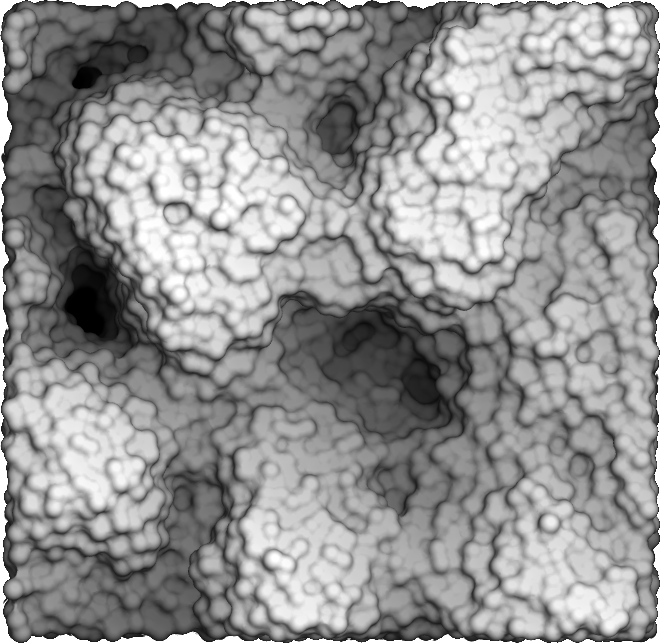
\includegraphics[width=\textwidth]{si111_surface_profile}
  \end{subfigure}
  \begin{subfigure}[t]{1.7cm}
    \def\svgwidth{\textwidth}
    \input{img/si111_surface_profile_halfscale.pdf_tex}
  \end{subfigure}
  \caption[Oberflächenprofil einer Silizium-PVD-Schicht]{Oberflächenprofil einer auf Si-(111) per PVD erzeugten Silizium-Schicht}
  \label{fig:siliconprofile}
\end{figure}

\begin{figure}[H]
  \centering
  \captionsetup[subfigure]{singlelinecheck=false}
  \begin{subfigure}[t]{7.1cm}
    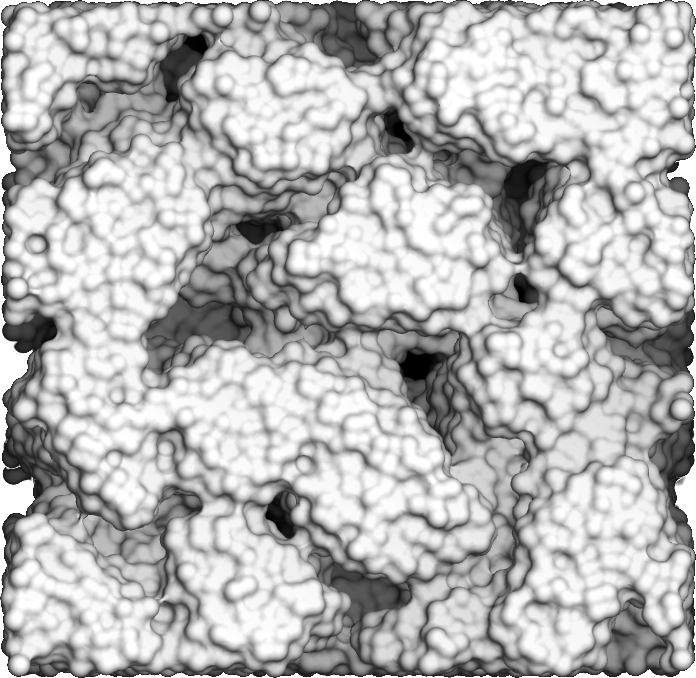
\includegraphics[width=\textwidth]{si111_underrelaxed_profile}
  \end{subfigure}
  \begin{subfigure}[t]{1.7cm}
    \def\svgwidth{\textwidth}
    \input{img/si111_underrelaxed_profile_scale.pdf_tex}
  \end{subfigure}
  \caption[Oberflächenprofil einer unterrelaxierten Siliziumschicht]{
    Oberflächenprofil einer unterrelaxierten Silizium-Schicht:
    Es bildet sich ein poröses Material mit Porentiefen oberhalb von \SI{6}{\nano\meter}, die linear mit der Schichtdicke wachsen
  }
  \label{fig:siliconunderrelaxedprofile}
\end{figure}
